\documentclass{article}

\usepackage{shyne}

% document format
\topmargin 0in
\oddsidemargin 0in
\evensidemargin 0in
\headheight 0in
\headsep 0in
\topskip 0in
\textheight 9in
\textwidth 6.5in
\linespread{1.3}

\begin{document}

\begin{flushleft}
\section*{Group Work - Week 10}

\paragraph{1} Conduct tests for the scenarios below at a $\alpha = 0.05$ level of significance. Be sure to state your conclusion in the context of the question.

\begin{enumalpha}
\item Researchers discover a new gene which, under the right circumstances, could lead to a mildly inconvenient, but chronic, disease. 10\% of the general population have the gene. One of the researchers thinks that people with naturally red hair have a different frequency of the gene. Genetic tests are conducted on a sample of 65 redheads and it is found that 11 of them have the gene. \\
\medskip
$\bv{H_0: p = 0.1}$\\
$\bv{H_0: p \ne 0.1}$\\
\medskip
\bt{The test statistic is $\bv{z= 1.861}$. The p-value is $\bv{p = 0.0628 > \alpha = 0.05}$. Do not reject the null hypothesis.\\
There is not evidence that redheads have a different frequency of the gene.}

\vspace{0.5in}

\item A coffee shop is interested in the proportion of decaf coffee drinkers on Sunday and Monday mornings. The manager thinks they have a lower proportion of decaf drinkers on Monday. They examine a random sample of coffee orders and find that on Sunday 52 out of 156 orders are for decaffeinated coffee and on Monday 43 out 174 are decaf orders. \\
\medskip
$\bv{H_0: p_1 - p_2 = 0}$\\
$\bv{H_0: p_1 - p_2 > 0}$\\
\medskip
\bt{From StatCrunch (Proportion Stats $\to$ Two Sample $\to$ With Summary):}\\
\bt{Z-stat: }$\bv{1.7267926}$\\
\bt{P-value: }$\bv{0.0421}$\\
\medskip

$\bv{z = 1.73, \, p = 0.0421 < \alpha = 0.05}$. \bt{Reject $\bv{H_0}$}.\\
\bt{There is evidence that the proportion of decaf coffee orders is lower on Mondays.}
\vspace{.5in}
\end{enumalpha}

\newpage
\paragraph{2} M\&Ms are expected to have the following distribution:\\
\smallskip
{\centering
\begin{tabular}{r | c c c c c c }
Color & Blue & Brown & Green & Orange & Red & Yellow\\
Percent & 24\% & 14\% & 15\% & 20\% & 13\% & 14\% 
\end{tabular}
\par} 
\begin{enumalpha}
\item What is the minimum number of M\&Ms needed to do a valid goodness-of-fit test against the expected distribution. In other words, what is the sample size $n$ so that the smallest expected value is at least 5?\\
\medskip
\bt{Since red is the least frequent color in the expected distribution, we need to find a sample size so that there are at least 5 expected red M\&M's.}\\
\medskip
$\ds\bv{n \times 0.13 \ge 5, \qquad n \ge \frac 5 {0.13} = 38.46}$\\
\medskip
\bt{So, the sample size should be at least 39 M\&M's.}
\vspace{.5in}
\item Conduct a goodness-of-fit test of whether the distribution of M\&Ms is what is claimed by the company at a significance level of $\alpha=0.05$. Make sure to state the null and alternative hypotheses, and your conclusion in context of question.\\
\medskip
\bt{(There are about 16 M\&M's in a regular fun size pack and about 7 M\&M's in a peanut fun size pack.)}\\
\medskip
\bt{The results will vary depending on the exact frequency of colors each finds.}\\
\bigskip
\bt{Example:}\\
\medskip
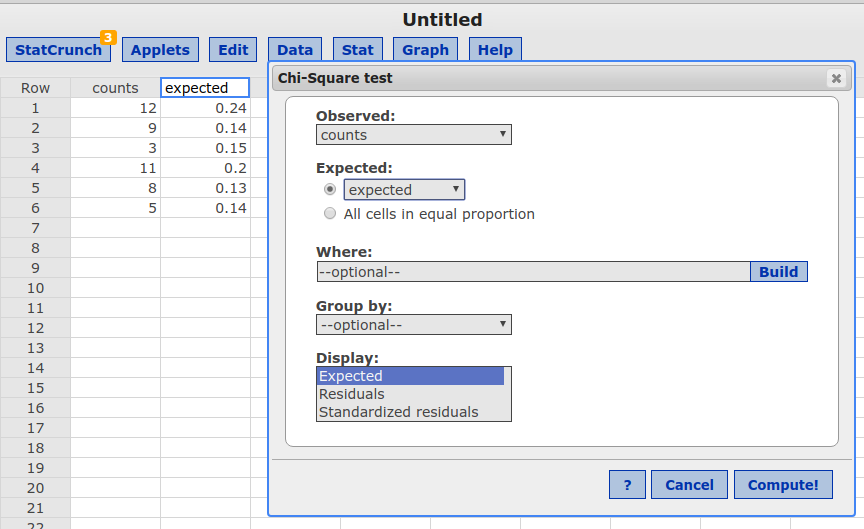
\includegraphics[width=4.5in]{images/group10_Q2_b}\\
$\bv{\chi^2 = 4.3843864, \, p = 0.4955 > \alpha = 0.05}$\\
\bt{Fail to reject $\bv{H_0}$. There is no evidence that M\&M colors don't follow the given distribution.}

\end{enumalpha}



\newpage
\paragraph{2} The Tortilla and Cheese Organization (TACO) thinks that preferences for types of tacos are the same for men and women. They conduct a survey and collect the following data (``taco\_preference.csv" on D2L):\\
\medskip
{\centering
\begin{tabular}{c | c  c c c}
\multicolumn{1}{c}{} & \multicolumn{4}{c}{\large Type of taco}\\
Gender & Beef & Pork & Chicken & Fish\\
\hline
Men & 105 & 34 & 56 & 27\\
Women & 83 & 29 & 75 & 35 \\
\end{tabular}
\par}
\bigskip
Test the claim the taco preference is the same for men and women at $\alpha = 0.05$ level of significance. Make sure to state the null and alternative hypotheses, and your conclusion in context of question.\\
\medskip
\bt{$\bv{H_0:}$ There is no association between gender and taco preference, or gender and taco preference are independent}\\
\bt{$\bv{H_a:}$ There is an association between gender and taco preference, or gender and taco preference are not independent}\\
\medskip
\bt{From StatCrunch (Tables $\to$ Contigency $\to$ With Summary):}\\
\bt{Value (Chi-square): }$\bv{6.7592767}$\\
\bt{P-value: }$\bv{0.08}$\\
\medskip

$\bv{\chi^2 = 6.76, \, p = 0.08 > \alpha = 0.05}$\\
\bt{Fail to reject $\bv{H_0}$. There is no evidence that taco preference and gender are not independent.}


\vspace{3.25in}



\end{flushleft}
\end{document}